\section*{Chapitre 2 - Droites et segments}
\addcontentsline{toc}{section}{Chapitre 2 - Droites et segments}
\subsection*{I. La droite}
\addcontentsline{toc}{subsection}{I. La droite}

\vspace{-0.3cm}
\subsubsection*{a. Alignement}
\addcontentsline{toc}{subsubsection}{a. Alignement}

\begin{Propriété*}
\begin{minipage}[c]{0.65\textwidth}

Par deux points distincts, il passe une unique droite. \\
Ici, on la note $(d)$, (AB) ou (BA).

\end{minipage}
\hfill
\begin{minipage}[c]{0.35\textwidth}
\begin{center}
\begin{tikzpicture}[scale=.6]
    % Droite orange (Couleur8) passant par B et A
    \draw[Couleur8, very thick] (-1.5,0.5) -- (3.5,-0.5);
    
     % A en haut
  \coordinate (B) at (0,0.2);
  % B au milieu
  \coordinate (A) at (2.5,-0.3);
  
    % Points B et A avec des croix
    
    \node[thick] at (0,0.2) {$+$};
    \node[thick] at (2.5,-0.3) {$+$};
    
    % Étiquettes des points
    \node[above] at (A) {A};
    \node[below left] at (B) {B};
    %\node at (0,0.7) {B};
    %\node at (2.5,0.3) {A};
    \node at (4,0) {$(d)$};
\end{tikzpicture}
\end{center}
\end{minipage}
\end{Propriété*}


\begin{minipage}[c]{0.8\textwidth}
\begin{Remarque}
\leavevmode\vspace{-\baselineskip}
\begin{itemize}[label=\textcolor{Couleur7}{$\bullet$}]
\item (AC) et (CB) sont par exemple d'autres noms de la droite (AB).
\item Une droite est composée d'une infinité de points.
\item On peut prolonger la droite (AB) au-delà de A et de B.
\end{itemize}
\end{Remarque}

\begin{Notation}
On dit que :
\begin{itemize}
\item le point C appartient à la droite $(d)$. On note : C $\in (d)$
\item le point D n'appartient pas à la droite $(d)$. On note : D $\notin (d)$

\end{itemize}
\end{Notation}

\end{minipage}
\hfill
\begin{minipage}[c]{0.15\textwidth}
\begin{center}
\begin{tikzpicture}[scale=0.6]

  % Droite (d) : presque verticale, légèrement inclinée
  % pente forte : de bas-droite vers haut-gauche
  \draw[Couleur6, thick] (-0.6, 3.2) -- (1.4, -1.8);
  \node[left, Couleur6] at (-0.6, 3.2) {$(d)$};

  % Points sur la droite (d)
  % A en haut
  \coordinate (A) at (-0.18, 2.2);
  % B au milieu
  \coordinate (B) at (0.6, 0.2);
  % C en bas à droite
  \coordinate (C) at (1.02, -0.8);

  % Point D : à gauche, pas sur la droite
  \coordinate (D) at (-0.8, 0.7);

  % --- Croix pour A, B, C, D ---
  \foreach \p in {A, B, C, D}{
    \draw[thick] ($(\p)+(-0.12,-0.12)$) -- ($(\p)+(0.12,0.12)$);
    \draw[thick] ($(\p)+(-0.12, 0.12)$) -- ($(\p)+(0.12,-0.12)$);
  }

  \node[above right] at (A) {A};
  \node[above right] at (B) {B};
  \node[right]       at (C) {C};
  \node[below left]       at (D) {D};

\end{tikzpicture}
\end{center}
\end{minipage}

\begin{Définition}[c]
On dit que des points sont alignés lorsqu'ils appartiennent à une même droite.
\end{Définition}
\subsubsection*{b. Positions de deux droites}
\addcontentsline{toc}{subsubsection}{b. Positions de deux droites}


% Figure 1 : droites parallèles
\newcommand{\figparalleles}{%
  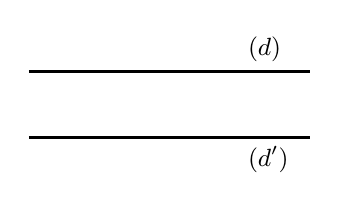
\begin{tikzpicture}[scale=0.7]
    \draw[thick] (-1.3,0.6) -- (3.8,0.6);
    \node[right] at (2.5,1) {\small $(d)$};
    \draw[thick] (-1.3,-0.6) -- (3.8,-0.6);
    \node[right] at (2.5,-1) {\small $(d')$};
  \end{tikzpicture}%
}


% Figure 2 : droites sécantes
\newcommand{\figsecantes}{%
  \begin{tikzpicture}[scale=0.7]
    % droite d (oblique de haut-gauche à bas-droite)
    \draw[thick] (-0.8, 1.4) -- (0.8,-1.4);
    \node[left] at (-0.8,1.4) {\small $(d)$};
    % droite d' (horizontale)
    \draw[thick] (-2,-0.5) -- (3,-0.5);
    \node[right] at (2,-1) {\small $(d')$};
    % point d'intersection O
    \coordinate (O) at (-0.3,-0.4);
    \node[below right,text=Couleur10] at (O) {\small O};
    % annotation "Point d'intersection"
    \node[align=center, text=Couleur10, font=\small\bfseries] at (1.5,1.5)
      {Point\\d'intersection};
    \draw[->, Couleur10, thick] (1,0.6) -- (0.3,-0.3);
  \end{tikzpicture}%
}

% Figure 3 : droites perpendiculaires
\newcommand{\figperp}{%
  \begin{tikzpicture}[scale=0.7]
      % codage de l'angle droit
    \draw[thick, Couleur7] (0,-0.3) rectangle (0.25,-0.05);
    % droite d (verticale)
    \draw[thick] (0,-0.9) -- (0,2);
    \node[above] at (-0.5,1.4) {\small $(d)$};
    % droite d' (horizontale)
    \draw[thick] (-0.5,-0.3) -- (4,-0.3);
    \node[right] at (2.9,-0.8) {\small $(d')$};
    % annotation "Codage de l'angle droit"
    \node[align=left, text=Couleur7, font=\small\bfseries] at (2.3,1.5)
      {Codage\\de l'angle droit};
    \draw[->, Couleur7, thick] (2.0,0.6) -- (0.3,0);
  \end{tikzpicture}%
}

\arrayrulecolor{Couleur6}
\renewcommand{\arraystretch}{1.2}

\begin{center}
\begin{tabular}{|>{\columncolor{Couleur6!10}}m{2.3cm}
                |>{\centering\arraybackslash\columncolor{white}}m{4.5cm}
                |>{\centering\arraybackslash\columncolor{white}}m{4.5cm}
                |>{\centering\arraybackslash\columncolor{white}}m{4.5cm}|}
\hline
\rowcolor{Couleur6!10}
Position & Droites parallèles & Droites sécantes & Droites perpendiculaires \\
\hline
Figure
  & \figparalleles
  & \figsecantes
  & \figperp \\
\hline
Définition
  & $(d)$ et $(d')$ ne se coupent jamais.
  & $(d)$ et $(d')$ se coupent au point O.
  & $(d)$ et $(d')$ se coupent en formant un angle droit. \\
\hline
Notation
  & $(d) \mathbin{/\!/} (d')$
  & Pas de notation
  & $(d) \perp (d')$ \\
\hline
\end{tabular}
\end{center}

\begin{Exemple}
\noindent
\begin{minipage}[c]{0.60\textwidth}
% --- ÉNONCÉ ---
\begin{enumerate}
\item Donner différents noms de la droite $(h)$.

\ligne

\ligne

\item Citer trois points alignés.


\ligne

\item Donner deux droites perpendiculaires.

\ligne


\item Donner deux droites parallèles : \ligne


\item Donner deux droites sécantes mais non perpendiculaires et préciser leur point d'intersection.

\ligne

\ligne


\end{enumerate}
\end{minipage}%
\hfill
% --- FIGURE ---
\begin{minipage}[c]{0.35\textwidth}
\usetikzlibrary{calc}

\begin{center}
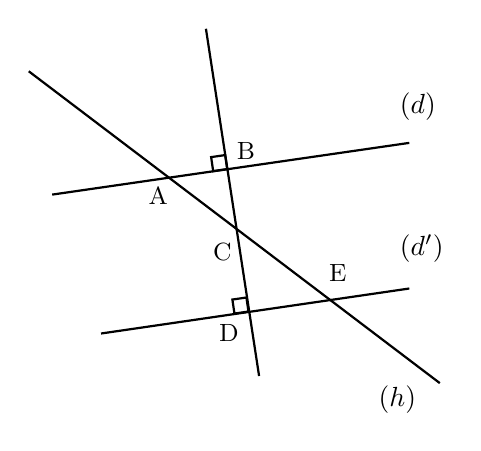
\begin{tikzpicture}[scale=0.9]
 
  \coordinate (B) at (0, 1.72);
  \coordinate (D) at (0.30, -0.34);


  \draw[thick]
    (B)
    -- ($(B) + 0.20*(-0.9895, -0.1443)$)
    -- ($(B) + 0.20*(-0.9895, -0.1443) + 0.20*(-0.1443,  0.9895)$)
    -- ($(B) + 0.20*(-0.1443,  0.9895)$)
    -- cycle;

  \draw[thick]
    ($(D) + (0, 0.05)$)
    -- ($(D) + 0.20*(-0.9895, -0.1443) + (0, 0.05)$)
    -- ($(D) + 0.20*(-0.9895, -0.1443) + 0.20*(-0.1443, 0.9895) + (0, 0.05)$)
    -- ($(D) + 0.20*(-0.1443, 0.9895) + (0, 0.05)$)
    -- cycle;
    
 
  \draw[thick] (-2.47, 1.36) -- (2.57, 2.09);
  \node[right] at (2.3, 2.6) {$(d)$};

 
  \draw[thick] (-1.78, -0.60) -- (2.57, 0.035);
  \node[right] at (2.3, 0.6) {$(d')$};

  \draw[thick] (-0.30, 3.70) -- (0.45, -1.20);

 
  \draw[thick] (-2.8, 3.1) -- (3, -1.3);
  \node[below right] at (2, -1.20) {$(h)$};

  % --- Recalcul des intersections ---

  \coordinate (A) at (-0.7, 1.6);

  \coordinate (C) at (0.2, 0.55);

  \coordinate (E) at (1.3, 0);



  \node[below left]       at (A) {\small A};
  \node[above right] at (B) {\small B};
  \node[left]        at (C) {\small C};
  \node[below left] at (D) {\small D};
  \node[above right]       at (E) {\small E};



\end{tikzpicture}
\end{center}
\end{minipage}%

\end{Exemple}

\newpage

\subsection*{II. Segment, demi-droite et milieu}
\addcontentsline{toc}{subsection}{II. Segment, demi-droite et milieu}


\begin{Définition*}
\begin{minipage}{0.6\textwidth}
Un \textbf{segment} est une partie de droite délimitée par deux points, appelés \textbf{extrémités} du segment. \\
On le note : [AB].
\end{minipage} \hfill
\begin{minipage}{0.35\textwidth}


\begin{tikzpicture}[scale=.9]
    % Ligne bleue horizontale qui s'étend au-delà des points A et B
    \draw[gray, thick] (-1,0) -- (5,0);
    
    % Segment AB en rouge
    \draw[Couleur6, ultra thick] (0,0) -- (4,0);
    
    % Points A et B avec des croix
    \node[Couleur1, thick] at (0,0) {I};
    \node[Couleur1, thick] at (4,0) {I};
    
    % Les étiquettes
    \node[Couleur1] at (0,-0.5) {A};
    \node[Couleur1] at (4,-0.5) {B};
    \node[Couleur6] at (2,-0.7) {Segment};
    \node[Couleur1] at (1.5,1) {Extrémités};
    
    % Flèches grises
    \draw[->, gray] (1.5,0.8) -- (0,0.2);
    \draw[->, gray] (1.5,0.8) -- (4,0.2);
    \draw[->, gray] (2,-0.5) -- (2,0);
\end{tikzpicture}

\end{minipage}
\end{Définition*}




\begin{Définition}
La \textbf{distance} entre deux points A et B est la longueur du segment [AB]. \\
Cette longueur est notée AB.
\end{Définition}

\begin{Définition*}
\begin{minipage}[c]{0.65\textwidth}
Lorsque l'on place un point C sur une droite (AB), on définit deux \textbf{demi-droites} d'origine C.

On note [CB) la demi-droite représentée en violet d'origine C passant par le point B. On note [CA) la demi-droite représentée en orange d'origine C passant par A.
\end{minipage}
\hfill
\begin{minipage}[c]{0.35\textwidth}
\begin{center}
\begin{tikzpicture}[scale=.9]
    % Droite orange (Couleur8) passant par B et A
    \draw[Couleur1, very thick] (-1.5,0) -- (1.7,0);
    \draw[Couleur10, very thick] (1.7,0) -- (3.5,0);
    
    % Points B et A avec des croix
    %\node[thick] at (0,0) {$+$};
    \node[thick] at (1.7,0) {I};
    %\node[thick] at (2.5,0) {$+$};
    
    \draw[thick] (-0.12,-0.12) -- (0.12,0.12);
    \draw[thick] (-0.12, 0.12) -- (0.12,-0.12);
    
    \draw[thick] (2.38,-0.12) -- (2.62,0.12);
    \draw[thick] (2.38, 0.12) -- (2.62,-0.12);
  
    % Étiquettes des points
    \node at (0,0.5) {B};
    \node at (1.7,0.5) {C};
    \node at (2.5,0.5) {A};
    \node at (-1.3,-0.5) {$(d)$};
\end{tikzpicture}
\end{center}
\end{minipage}
\end{Définition*}





\begin{Exemple}
\begin{minipage}{0.7\textwidth}
Nommer une droite, une demi-droite, un segment et sa longueur. \\

Droite : $\ldots\ldots$\\[2mm]
Demi-droite : $\ldots\ldots$\\[2mm]
Segment : $\ldots\ldots$\\[2mm]
Longueur : $\ldots\ldots$\\[2mm]


\end{minipage} \hfill
\begin{minipage}{0.3\textwidth}
\begin{tikzpicture}[scale=0.8,rotate=20]

  % Points
  \coordinate (A) at (0,0);
  \coordinate (B) at (2,0);
  \coordinate (C) at (0,2);
  \coordinate (D) at (2,-0.75);

  % Angles droits
  \draw[Couleur7] (0,0) rectangle ++(0.2,0.2);   % angle droit en A
  \draw[Couleur7] (2,0) rectangle ++(-0.2,0.2);  % angle droit en B (vers la gauche)
  
  % Droite (CA) prolongée au-delà de C
  \draw (A) -- ($(C)!1.3!(A) + (C) - (A)$);
  \draw (A) -- (C);
  \draw[shorten >=-0.8cm] (A) -- (C);

  % On trace la droite CA prolongée vers le haut
  \draw (A) -- ++(0,1.5);

  % Droite AB
  \draw (A) -- (B) node[midway, below, rotate = 20] {5 cm};

  % Droite (BD) prolongée
  \draw (B) -- ++(0,1.5);
  \draw (B) -- ++(0,-1.5);



  % Tirets de parallélisme sur (CA) et (BD)
  \draw ($(A)!1!(C) + (-0.12,0)$) -- ($(A)!1!(C) + (0.12,0)$);
  \draw ($(B)!1!(D) + (-0.12,0)$) -- ($(B)!1!(D) + (0.12,0)$);

  % Labels
  \node[left]  at (C)  {C};
  \node[left]  at (A)      {A};
  \node[right] at (B)      {B};
  \node[right] at (D) {D};

\end{tikzpicture}
\end{minipage}

\end{Exemple}



\begin{Exemple}

\begin{minipage}{0.55\textwidth}
Compléter par $\in$ ou $\notin$ :
\begin{multicols}{2}
\begin{itemize}
\item $U \ldots [XV)$
\item $X \ldots [VO)$
\item $V \ldots (XP)$
\item $X \ldots [VP]$ 
\item $V \ldots [OX)$
\item $O \ldots [UV]$ 
\end{itemize}
\end{multicols}
\end{minipage} \hfill
\begin{minipage}{0.45\textwidth}
\begin{center}
 \begin{tikzpicture}[baseline,scale = 0.5]

    \tikzset{
      point/.style={
        thick,
        draw,
        cross out,
        inner sep=0pt,
        minimum width=5pt,
        minimum height=5pt,
      },
    }
    \clip (-1,-4) rectangle (12,2);
    	\draw[color ={black},line width = 0.625,opacity = 0.8] (-0.19,0.19)--(0.19,-0.19);
    	\draw[color ={black},line width = 0.625,opacity = 0.8] (-0.19,-0.19)--(0.19,0.19);
    	\draw[color ={black},line width = 0.625,opacity = 0.8] (10.81,-1.81)--(11.19,-2.19);
    	\draw[color ={black},line width = 0.625,opacity = 0.8] (10.81,-2.19)--(11.19,-1.81);
    %	\draw[color ={black},line width = 0.625,opacity = 0.8] (3.81,3.19)--(4.19,2.81);
    	%\draw[color ={black},line width = 0.625,opacity = 0.8] (3.81,2.81)--(4.19,3.19);
    %	\draw[color ={black},line width = 0.625,opacity = 0.8] (7.81,-6.81)--(8.19,-7.19);
    %\draw[color ={black},line width = 0.625,opacity = 0.8] (7.81,-7.19)--(8.19,-6.81);
    \draw[color ={black},line width = 0.625,opacity = 0.8] (0.81,0.01)--(1.19,-0.37);\draw[color ={black},line width = 0.625,opacity = 0.8] (0.81,-0.37)--(1.19,0.01);\draw[color ={black},line width = 0.625,opacity = 0.8] (3.81,-0.54)--(4.19,-0.91);\draw[color ={black},line width = 0.625,opacity = 0.8] (3.81,-0.91)--(4.19,-0.54);
   % \draw[color ={black},line width = 0.625,opacity = 0.8] (6.81,-1.09)--(7.19,-1.46);
   % \draw[color ={black},line width = 0.625,opacity = 0.8] (6.81,-1.46)--(7.19,-1.09);
    \draw[color ={black},line width = 0.625,opacity = 0.8] (8.81,-1.45)--(9.19,-1.82);\draw[color ={black},line width = 0.625,opacity = 0.8] (8.81,-1.82)--(9.19,-1.45);
	\draw [color={black}] (-0.5,0.6) node[anchor = center,scale=1, rotate = 0] {O};
	\draw [color={black}] (11.5,-1.6) node[anchor = center,scale=1, rotate = 0] {P};
	
	\draw [color={black}] (1,-0.8) node[anchor = center,scale=1, rotate = 0] {U};
	\draw [color={black}] (4,-1.3) node[anchor = center,scale=1, rotate = 0] {V};
	\draw [color={black}] (7,-9) node[anchor = center,scale=1, rotate = 0] {W};
	\draw [color={black}] (9,-2.2) node[anchor = center,scale=1, rotate = 0] {X};
	\draw[color=Couleur6, thick] (-49.193495504995376,8.94427190999916)--(60.193495504995376,-10.94427190999916);
	

\end{tikzpicture}
\end{center}
\end{minipage}

\end{Exemple}


\begin{Définition*}
\begin{minipage}{0.6\textwidth}
Le \textbf{milieu} d'un segment est le point qui appartient à ce segment et qui est à égale distance des extrémités de ce segment.
\end{minipage} \hfill
\begin{minipage}{0.35\textwidth}
\begin{tikzpicture}[scale=.9]
    % Ligne horizontale bleue
    \draw[Couleur10, very thick] (0,0) -- (5,0);
    
    % Points S, J, T avec des croix
    \node[thick] at (0,0) {I};
    \node[thick] at (2.5,0) {I};
    \node[thick] at (5,0) {I};
    
    % Étiquettes des points
    \node at (0,0.5) {S};
    \node at (2.5,0.5) {J};
    \node at (5,0.5) {T};
    
    % Doubles traits obliques et plus petits pour indiquer l'égalité des segments
    \draw[gray, thick] (1.15,-0.1) -- (1.35,0.1);
    \draw[gray, thick] (1.25,-0.1) -- (1.45,0.1);
    
    \draw[gray, thick] (3.55,-0.1) -- (3.75,0.1);
    \draw[gray, thick] (3.65,-0.1) -- (3.85,0.1);
    
    % Double flèche arquée rouge pour indiquer l'égalité, positionnée plus haut
    \draw[<->, Couleur8, thick] (1.25,-0.4) to[out=-30,in=-150] (3.75,-0.4);
    
    % Texte explicatif
    \node at (2.5,-1.2) {Codage indiquant que JS = JT.};
\end{tikzpicture}


\end{minipage}

\end{Définition*}


\begin{Exemple}
Sur la figure ci-dessus, le point J est équidistant (à égale distance) de S et de T et il appartient au segment [ST] : J est donc le milieu de [ST].
\end{Exemple}
\vspace{0.2cm}
\begin{Remarque}
\leavevmode\vspace{-\baselineskip}
Une droite est illimitée : elle n'a ni longueur ni milieu.
\end{Remarque}



